\section{Methodology}
\label{sec:methodology}

\vspace{-2mm}

We formalize LLM--agent collaboration as autoregressive generation over a mixed-modality trace of \lang{language}, \action{action}, and \state{state} tokens. This formulation isolates the \emph{integration interface}---how the agent's internal state enters the LLM's reasoning---as a single controlled variable, and connects directly to the reinforcement learning objective that optimizes it.

\subsection{Formulation}
\label{sec:formulation}

A policy $\pi_\theta$ (the LLM) collaborates with a pretrained domain agent whose encoder $G_\psi\!: \mathcal{S} \to \R^d$ maps environment states to latent representations $\vh_s = G_\psi(s)$.
Over a $T$-step interaction, $\pi_\theta$ generates a trace interleaving three token types: \mlang{language tokens} $w_t \in \mathcal{V}$ for verbal reasoning, \maction{action tokens} $a_t \in \mathcal{A}$ for environment interaction, and \mstate{state tokens} $\vz_t \in \R^{k \times e}$ carrying the agent's projected latent representation.
At decision-relevant moments, $\pi_\theta$ issues a structured tool call to the agent, which processes the current state $s_t$ and injects $k$ contiguous \state{state tokens} into the trace (\S\ref{sec:invocation}).
The agent re-encodes the updated state at each invocation, so $\mstate{\vz_t}$ reflects the environment after prior actions---a closed loop between reasoning and perception, where both the timing and target state of invocations are optimized by reinforcement learning.
The complete trace takes the form:
%
\begin{equation}
\tau = \bigl(\,
  \mlang{w_{1:j_1}},\;
  \mstate{\vz_1^{1:k}},\;
  \maction{a_1},\;
  \mlang{w_{j_1\!+\!1:j_2}},\;
  \mstate{\vz_2^{1:k}},\;
  \maction{a_2},\;
  \ldots,\;
  \mstate{\vz_T^{1:k}},\;
  \maction{a_T},\;
  \mlang{w_{\mathrm{final}}}
\,\bigr)
\label{eq:trace}
\end{equation}
%
where $\pi_\theta$ generates \mlang{language} and \maction{action} tokens autoregressively; \mstate{state} tokens are injected by the agent and carry no token distribution.

\paragraph{Integration interface.}
The agent's latent representation $\vh_s \in \R^d$ encodes its policy distribution, value estimates, and learned features~\cite{jenner2024evidence}. How this representation enters the trace defines the \textbf{integration interface}---the sole variable our experiments control:
%
\begin{align}
\text{Verbalized:}~~  & \mstate{\hat{w}_t} = \mathrm{Verb}\bigl(G_\psi(s_t)\bigr) \in \mathcal{V}^*, \label{eq:verb_channel} \\[2pt]
\text{Internalized:}~~& \mstate{\vz_t}\;\, = H_\varphi\bigl(G_\psi(s_t)\bigr) \in \R^{k \times e}. \label{eq:latent_channel}
\end{align}
%
Verbalization compresses $\R^d$ to a discrete token string---a lossy channel that collapses distributional structure into surface-level descriptions (e.g., ``best move: Nc2, eval: $+0.3$'').
The text rendering $\mathrm{Verb}$ can range from sparse (top-1 move) to dense (full policy distribution serialized as text); we ablate across this spectrum in \S\ref{sec:experiments}.
Internalization projects $\R^d$ to the LLM's embedding space via a learned mapping $H_\varphi$, optimized end-to-end with the policy through reinforcement learning.

\paragraph{The controlled contrast.}
Under matched backbone, reward, and rollout budget, the integration interface enters the objective through exactly one term---the conditioning of the importance ratio. Writing $y_t$ for the generated token at position $t$ (language or action):
%
\begin{align}
r_t^{\,\mathrm{verb}} &=
  \frac{\pi_\theta\bigl(y_t \mid y_{<t},\; \mstate{\hat{w}_{<t}}\bigr)}
       {\pi_{\theta_{\mathrm{old}}}\bigl(y_t \mid y_{<t},\; \mstate{\hat{w}_{<t}}\bigr)},
  &\mstate{\hat{w}} &= \mathrm{Verb}(G_\psi(s)),  \label{eq:ratio_verb} \\[4pt]
r_t^{\,\mathrm{latent}} &=
  \frac{\pi_\theta\bigl(y_t \mid y_{<t},\; \mstate{\vz_{<t}}\bigr)}
       {\pi_{\theta_{\mathrm{old}}}\bigl(y_t \mid y_{<t},\; \mstate{\vz_{<t}}\bigr)},
  &\mstate{\vz} &= H_\varphi(G_\psi(s)). \label{eq:ratio_latent}
\end{align}
%
This yields two testable quantities: the \textbf{Verbalization Gap} $\mathrm{VG}(\mathcal{T}) = \sigma_{\mathrm{latent}}(\mathcal{T}) - \sigma_{\mathrm{verb}}(\mathcal{T})$ measuring the per-task performance difference, and the \textbf{Depth-Compounding Slope (DCS)}---the rate at which VG grows with interaction depth across the benchmark.
We hypothesize $\mathrm{VG} > 0$ and that the gap compounds: tasks requiring deeper multi-step collaboration expose larger gaps than single-step perception tasks.

\subsection{Architecture}
\label{sec:architecture}

\textbf{Pretrained Agent.}
We instantiate $G_\psi$ with Lc0-BT4~\cite{monroe2024mastering}, a 15-layer Transformer encoder (240\,M parameters) whose representations encode positional features and implicit planning signals~\cite{jenner2024evidence}, producing $\vh_s \in \R^{1024}$.

\textbf{Large Language Model.}
We use Qwen3~\cite{XXXqwen3} as the backbone $\pi_\theta$. To accept \mstate{state tokens} from the agent, we follow the multimodal alignment approach of LLaVA~\cite{liu2023visual}: $k$ contiguous token positions in the input sequence serve as placeholders whose embeddings are replaced by the projected agent state $\vz_s$.

\textbf{Projector.}
The mapping $H_\varphi\!: \R^{d} \to \R^{k \times e}$ (Eq.~\ref{eq:latent_channel}) is a three-layer MLP with GeLU activation, projecting the agent's $d$-dimensional latent state into $k$ embeddings of dimension $e$ matching the LLM's hidden size. As illustrated in Figure~\ref{fig:LLAMIA}, the resulting input is a mixed sequence $[\mlang{w_1}, \mstate{\vz_s^{1:k}}, \maction{a_1}, \mlang{w_2}]$, allowing the LLM to attend jointly to all three modalities.

\subsection{Training}
\label{sec:training}

Training proceeds in two stages. Stage~1 grounds the agent's latent representations in the LLM's embedding space via supervised learning with the LLM frozen. Stage~2 trains the full system---LLM and projector jointly---via reinforcement learning on mixed-modality rollouts.

\begin{figure}[!h]
    \centering
    \vspace{-8mm}
    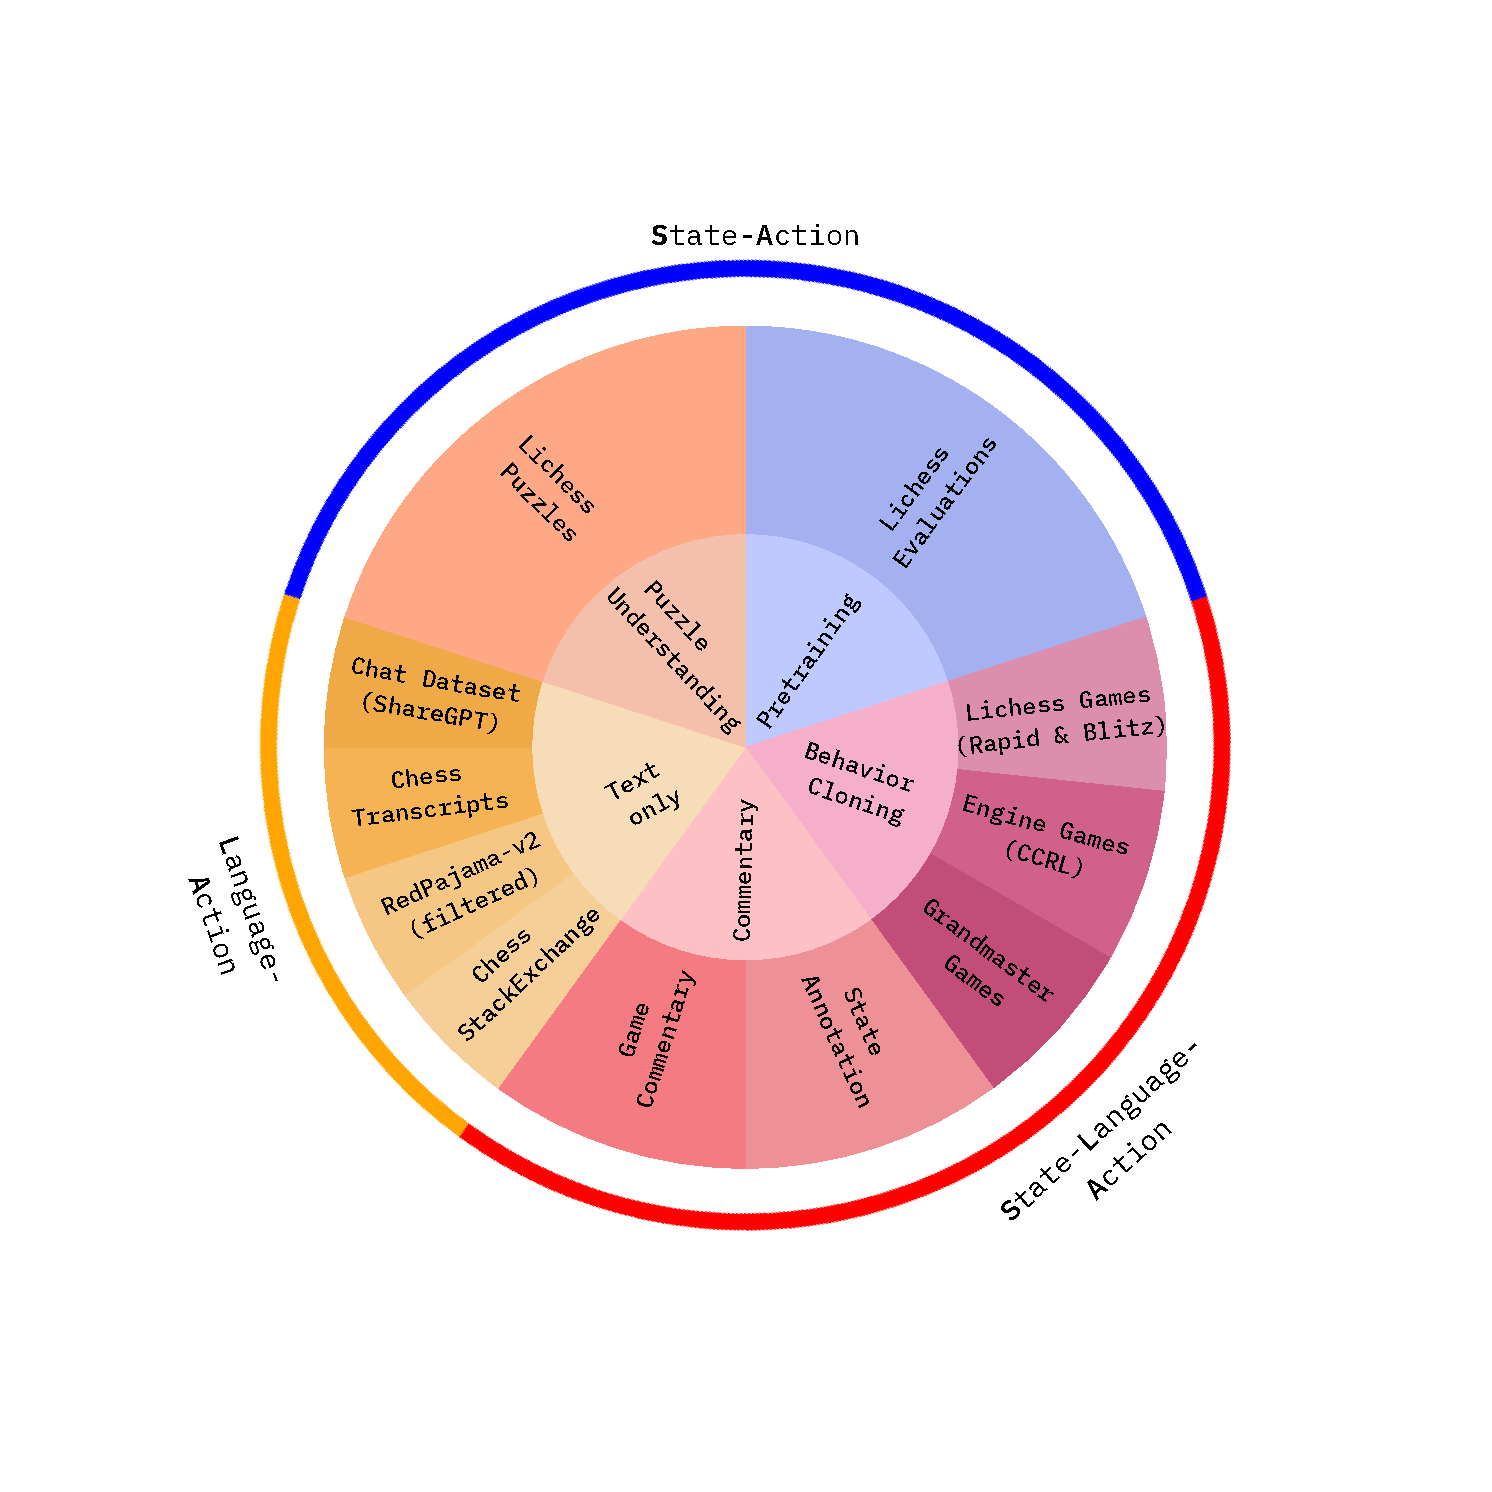
\includegraphics[width=0.98\linewidth]{data.pdf}
    \vspace{-8mm}
    \caption{The inner circle represents the distribution of training data, detailing the categories. The outer circle lists the types and data sources present in each category.}
    \label{fig:data}
\end{figure}

\begin{figure}[!h]
    \centering
    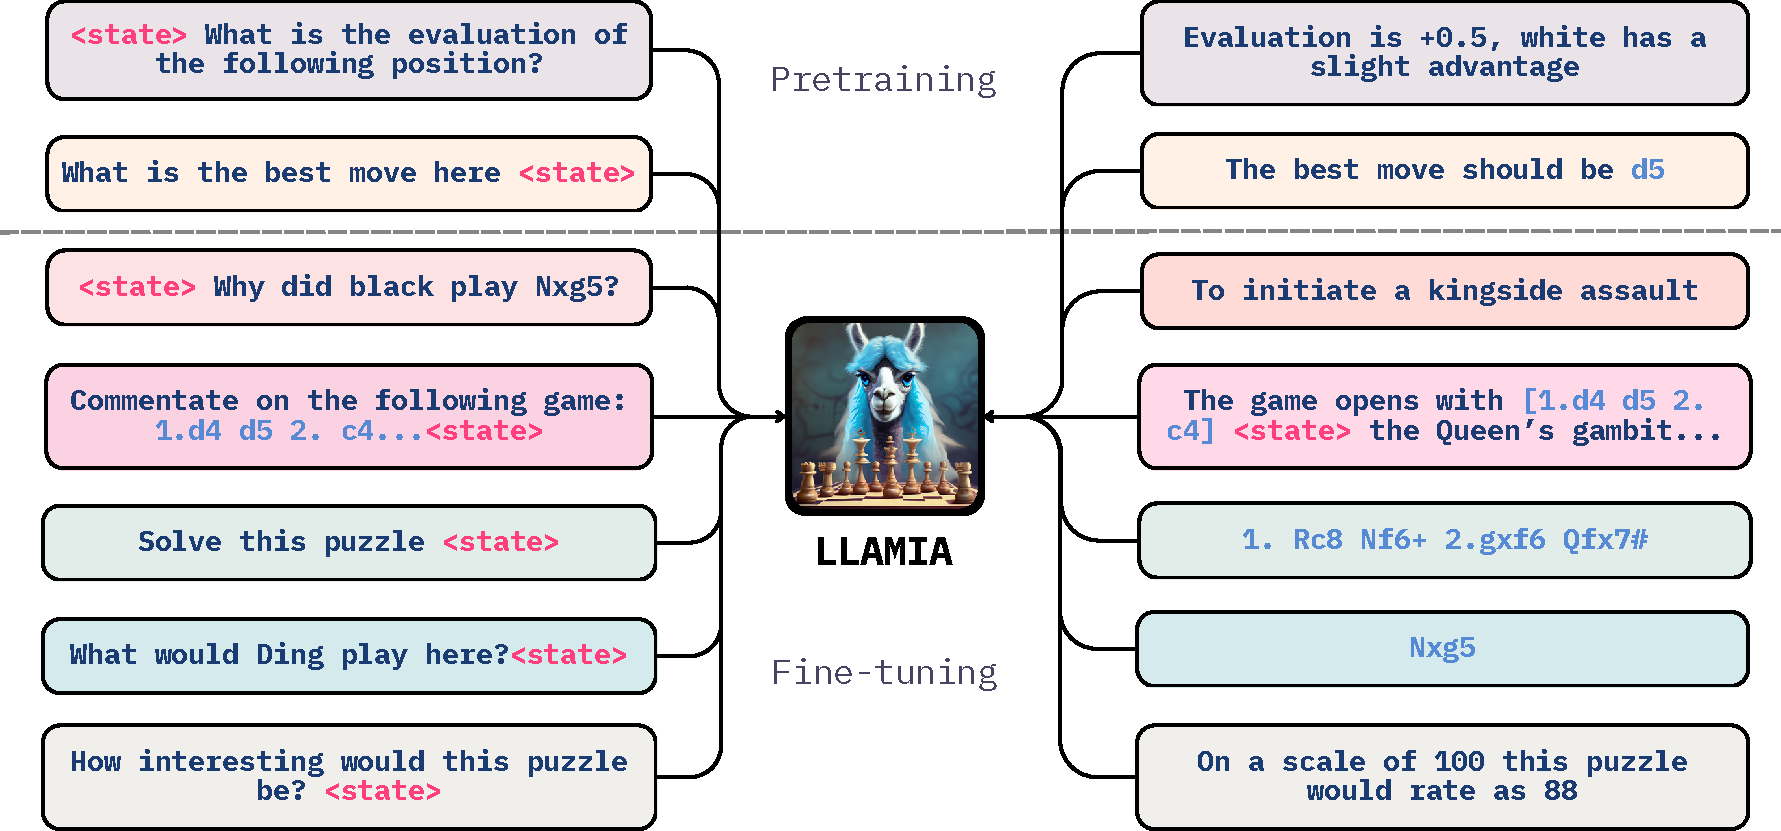
\includegraphics[width=0.98\linewidth]{llamia-tasks3.pdf}
    \caption{Tasks demonstrating LLAMIA capabilities across planning, reasoning, and acting: chess evaluations, best move predictions, behavior cloning, commentary prediction, state annotation, and puzzle understanding.}
    \label{fig:LLAMIA-arch-tasks}
\end{figure}

\subsubsection{Stage 1: Projector Alignment}
\label{sec:stage1}

We train only the projection network $H_\varphi$ to align the agent's latent representations $\vh_s$ with the LLM's token embedding space, while keeping the language model $\pi_\theta$ frozen. We construct a large-scale dataset $\mathcal{D}_{\text{pre}} = \{(s, \pi(s))\}$ by sampling state-policy pairs from the pretrained agent's self-play. Each example is paired with a language prompt (e.g., ``Analyze position: top move?''), and the model learns to generate the correct action token corresponding to $\pi(s)$. The exact prompt format is given in Listing~\ref{listing:pretraining_instruction_format}. Training minimizes the cross-entropy loss:
\[
\mathcal{L}_{\text{Stage\,1}} = -\mathbb{E}_{(s, \pi(s)) \sim \mathcal{D}_{\text{pre}}} \log \pi_\theta\!\left( \pi(s) \mid \vz_s, \text{prompt} \right)
\]
Because the LLM is frozen, the projector can be trained on abundant agent-generated data without risking catastrophic interference with language modeling.

\subsubsection{Stage 2: Reinforcement Learning}
\label{sec:stage2}

The second stage unfreezes both the LLM $\pi_\theta$ and the projector $H_\varphi$, and optimizes them jointly via DAPO~\cite{XXXdapo}. Rollouts produce complete mixed-modality traces $\tau$ (Eq.~\ref{eq:trace}); the policy gradient operates over positions where the LLM generates---\mlang{language} and \maction{action} tokens---while \mstate{state} positions are agent-injected and excluded from the gradient:
%
\begin{equation}
J(\theta, \varphi) \!=\! \mathbb{E}_{\tau \sim \pi_{\theta_{\mathrm{old}}}} \!\Bigg[\!
  \frac{1}{|\mathcal{I}_{\mathrm{gen}}|}
  \!\!\sum_{t \,\in\, \mlang{\mathcal{I}_{L}} \,\cup\, \maction{\mathcal{I}_{A}}}
  \!\!\min\!\Big(
    r_t\,\hat{A}_t,\,
    \mathrm{clip}(r_t, 1\!-\!\varepsilon_l, 1\!+\!\varepsilon_h)\,\hat{A}_t
  \Big)
\Bigg]
\label{eq:dapo}
\end{equation}
%
where $\hat{A}_t$ is the group-normalized advantage and the asymmetric clip bounds $\varepsilon_l \leq \varepsilon_h$ encourage exploration~\cite{XXXdapo}. The reward decomposes as $\mathcal{R}(\tau) = R_{\mathrm{outcome}} + R_{\mathrm{format}} + R_{\mathrm{collab}}$, combining task performance, syntactic validity, and a collaboration-shaping signal; full definitions are given in Appendix~\ref{sec:app_reward}.

Because the projector $H_\varphi$ is now unfrozen, the RL objective optimizes the integration interface end-to-end: gradients flow from the reward through the LLM's generated tokens back to the projector, shaping \emph{how} the agent's latent state is presented to the LLM---not just how the LLM uses it.

\subsubsection{Agent Invocation}
\label{sec:invocation}

LLAMIA invokes the agent through a structured tool call that the LLM learns to emit during RL. The call specifies a state---either the current environment state or a counterfactual state reached by a hypothetical action---and the agent encodes the specified state via $G_\psi$. The projector maps the result to $k$ latent tokens via $H_\varphi$, which are inserted into the trace, after which the LLM resumes autoregressive generation.

This mechanism creates a closed loop: the LLM reasons in language, acts on the environment, and queries the agent for a fresh encoding of the resulting state. Crucially, RL optimizes not only what the LLM does with the agent's response but also \emph{when} and \emph{whether} it invokes the agent---the invocation itself is part of the policy's action space. We show in \S\ref{sec:experiments} that removing dynamic re-encoding degrades multi-step tasks by 64\% while leaving single-step perception tasks largely unaffected (1--4\%), confirming that learned invocation timing is essential for sustained collaboration.
